\documentclass[a4paper,fleqn]{article}
\usepackage[margin=1in]{geometry} % Sets all margins to 1 inch

\usepackage{graphicx} % Required for inserting images
\usepackage{subfig}
\usepackage{units}
\usepackage[numbers]{natbib}
% \usepackage{gensymb}
\usepackage{caption}
\usepackage{enumitem}
\usepackage{units}
\usepackage[x11names]{xcolor}
\usepackage{amsmath}
\usepackage{booktabs}
\usepackage{enumitem}
\usepackage{physics}
\usepackage{float}

\usepackage{hyperref}
\hypersetup{
    colorlinks=true,
    linkcolor=black,    
    urlcolor=cyan,
    citecolor= blue,
}

\newcommand{\file}[1]{\textcolor{brown}{\texttt{#1}}}
\newcommand{\type}[1]{\textcolor{blue}{\texttt{#1}}}
\newcommand{\class}[1]{\textcolor{Green3}{\texttt{#1}}}
\newcommand{\function}[1]{\textcolor{orange}{\texttt{#1}}}



\title{OpenLPT Document}
\author{Shijie Zhong, Han Zheng}
\date{}

\begin{document}

\maketitle
\thispagestyle{empty}
\tableofcontents
\vfill
\begin{minipage}{14cm}{
\small \sffamily
Version: 1.0.0 \\
Last updated: \today  \\
Github repository: \url{https://github.com/clockj/OpenLPTGUI} \\
Contact the developers: szhong12@jhu.edu
 }
\end{minipage}

\newpage
\pagenumbering{arabic}


%          %
% Sections %
%          %
\section{Introduction}


In experimental fluid dynamics, flow velocity is often measured by tracking small tracer particles that follow the flow accurately \citep{nishino1989three,papantoniou1989analyzing}. Lagrangian particle tracking is widely used for this purpose, as it provides longer particle trajectories than other methods, making it ideal for studying particle dispersion and mixing \citep{barta2024proptv,schanz2016shake,tan2020introducing,shnapp2022myptv}. This technique reconstructs 3D particle positions from synchronized camera images and links them across frames to generate trajectories. Algorithms like iterative particle reconstruction and shake-the-box further enhance accuracy and trajectory length \citep{wieneke2012iterative, schanz2016shake}. While the original \textit{OpenLPT} code, available on GitHub, is optimized, it is written in C++ without an easy-to-use interface. This repository presents an updated version with a user-friendly GUI and Python API, improving accessibility for the scientific community.


\textit{pyOpenLPT} is a Python package for 3D Lagrangian particle tracking, built on \textit{OpenLPT}. The core C++ code is optimized for tracking large numbers of particles ($\sim O(5\times10^4)$) and includes new features like a polynomial camera model, better calibration, and support for different camera setups. The new code is modular, making it easier to add new features such as object identification and multi-object tracking. \textit{pyOpenLPT} provides a user-friendly Python interface for the efficient C++ code and can be easily installed on both Windows and Linux.


The \textit{pyOpenLPT} GUI, called \textit{OpenLPTGUI}, provides a simple, user-friendly interface for applying Lagrangian particle tracking to flow measurement. It offers a clear, step-by-step workflow with included documentation. The process covers calibration point extraction, camera calibration, image preprocessing, tracking, and camera parameter optimization.


The \textit{OpenLPT} code family, including \textit{pyOpenLPT} and \textit{OpenLPTGUI}, has been used in several scientific publications \citep{salibindla2020lift,qi2020towards,masuk2021simultaneous,salibindla2021experimental,masuk2021orientational,masuk2021towards,qi2022fragmentation,tan2022universality,tan2023scalings}. With the latest version, the software is now more accessible to the experimental community, allowing more researchers to achieve high-quality 3D flow measurements and make new discoveries.



\section{Installation}

Users can refer to \url{https://github.com/clockj/OpenLPTGUI} and \url{https://github.com/clockj/OpenLPT} for details of installation.


\section{OpenLPT Workflow}

OpenLPT workflow includes five steps: (1) calibration method selection ("1. Select a calibration method"); (2) camera model selection ("2. Select a camera model"); (3) image preprocessing ("3. Preprocess images (Optional)"); (4) tracking ("4. Run OpenLPT"); and (5) refine camera parameters ("5. Run volume self calibration (Optional, suggested for few calibration points)"). 
After entering the main page of OpenLPTGUI, users can follow the workflow according to the step number as shown in Fig.\ref{fig:GUI_main}. 

\begin{figure}[h]
    \centering
    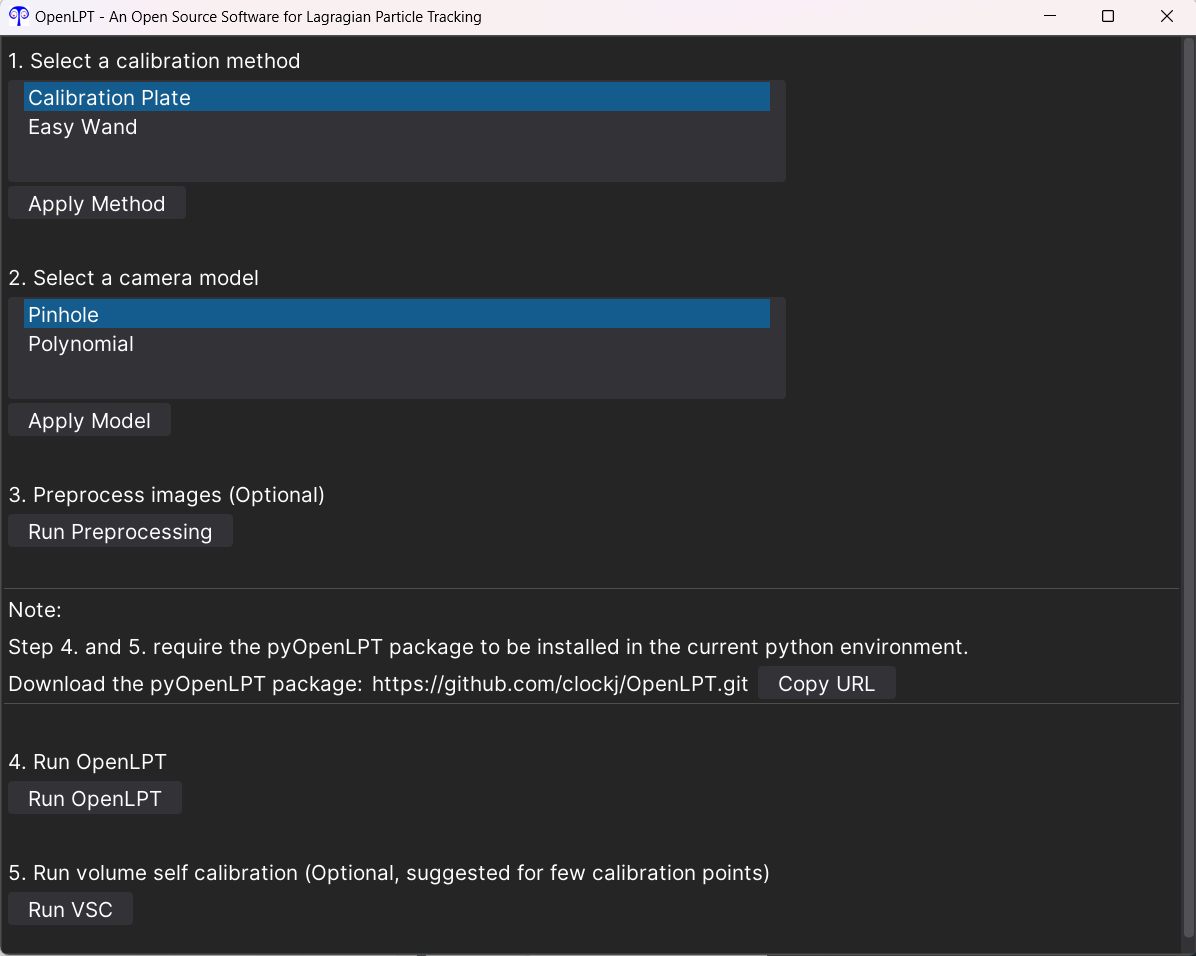
\includegraphics[width=\linewidth]{Fig/GUI_main.png}
    \caption{OpenLPTGUI main page.}
    \label{fig:GUI_main}
\end{figure}


\subsection{Calibration Method Selection}
In this step, the goal is to extract the 2D coordinates of calibration points on each camera and the corresponding 3D positions. It should be done for each image taken for calibration. The \textit{Calibration Plate} method refers to using calibration plate with circular dots for calibration. Users can put the calibration plates at different planes for calibration, but the same procedure should be repeated for extracting points on each plane. The \textit{Easy Wand} method refers to using a calibration rod that moves randomly in the field of view for calibration \citep{theriault2014protocol}. The calibration rod involves two different sized spherical ball on the two ends. However, this method is not supported in this version but will be implemented in the future.

\begin{enumerate}
    \item Calibration Plate
    \begin{enumerate}
        \item \textit{Import}\\
    Import a photo (8 bits) of the calibration plate by clicking "Import Image". A sample image is located at \file{images/cam1frame\_Z0.tif}. 
    \begin{figure}[h]
        \centering
        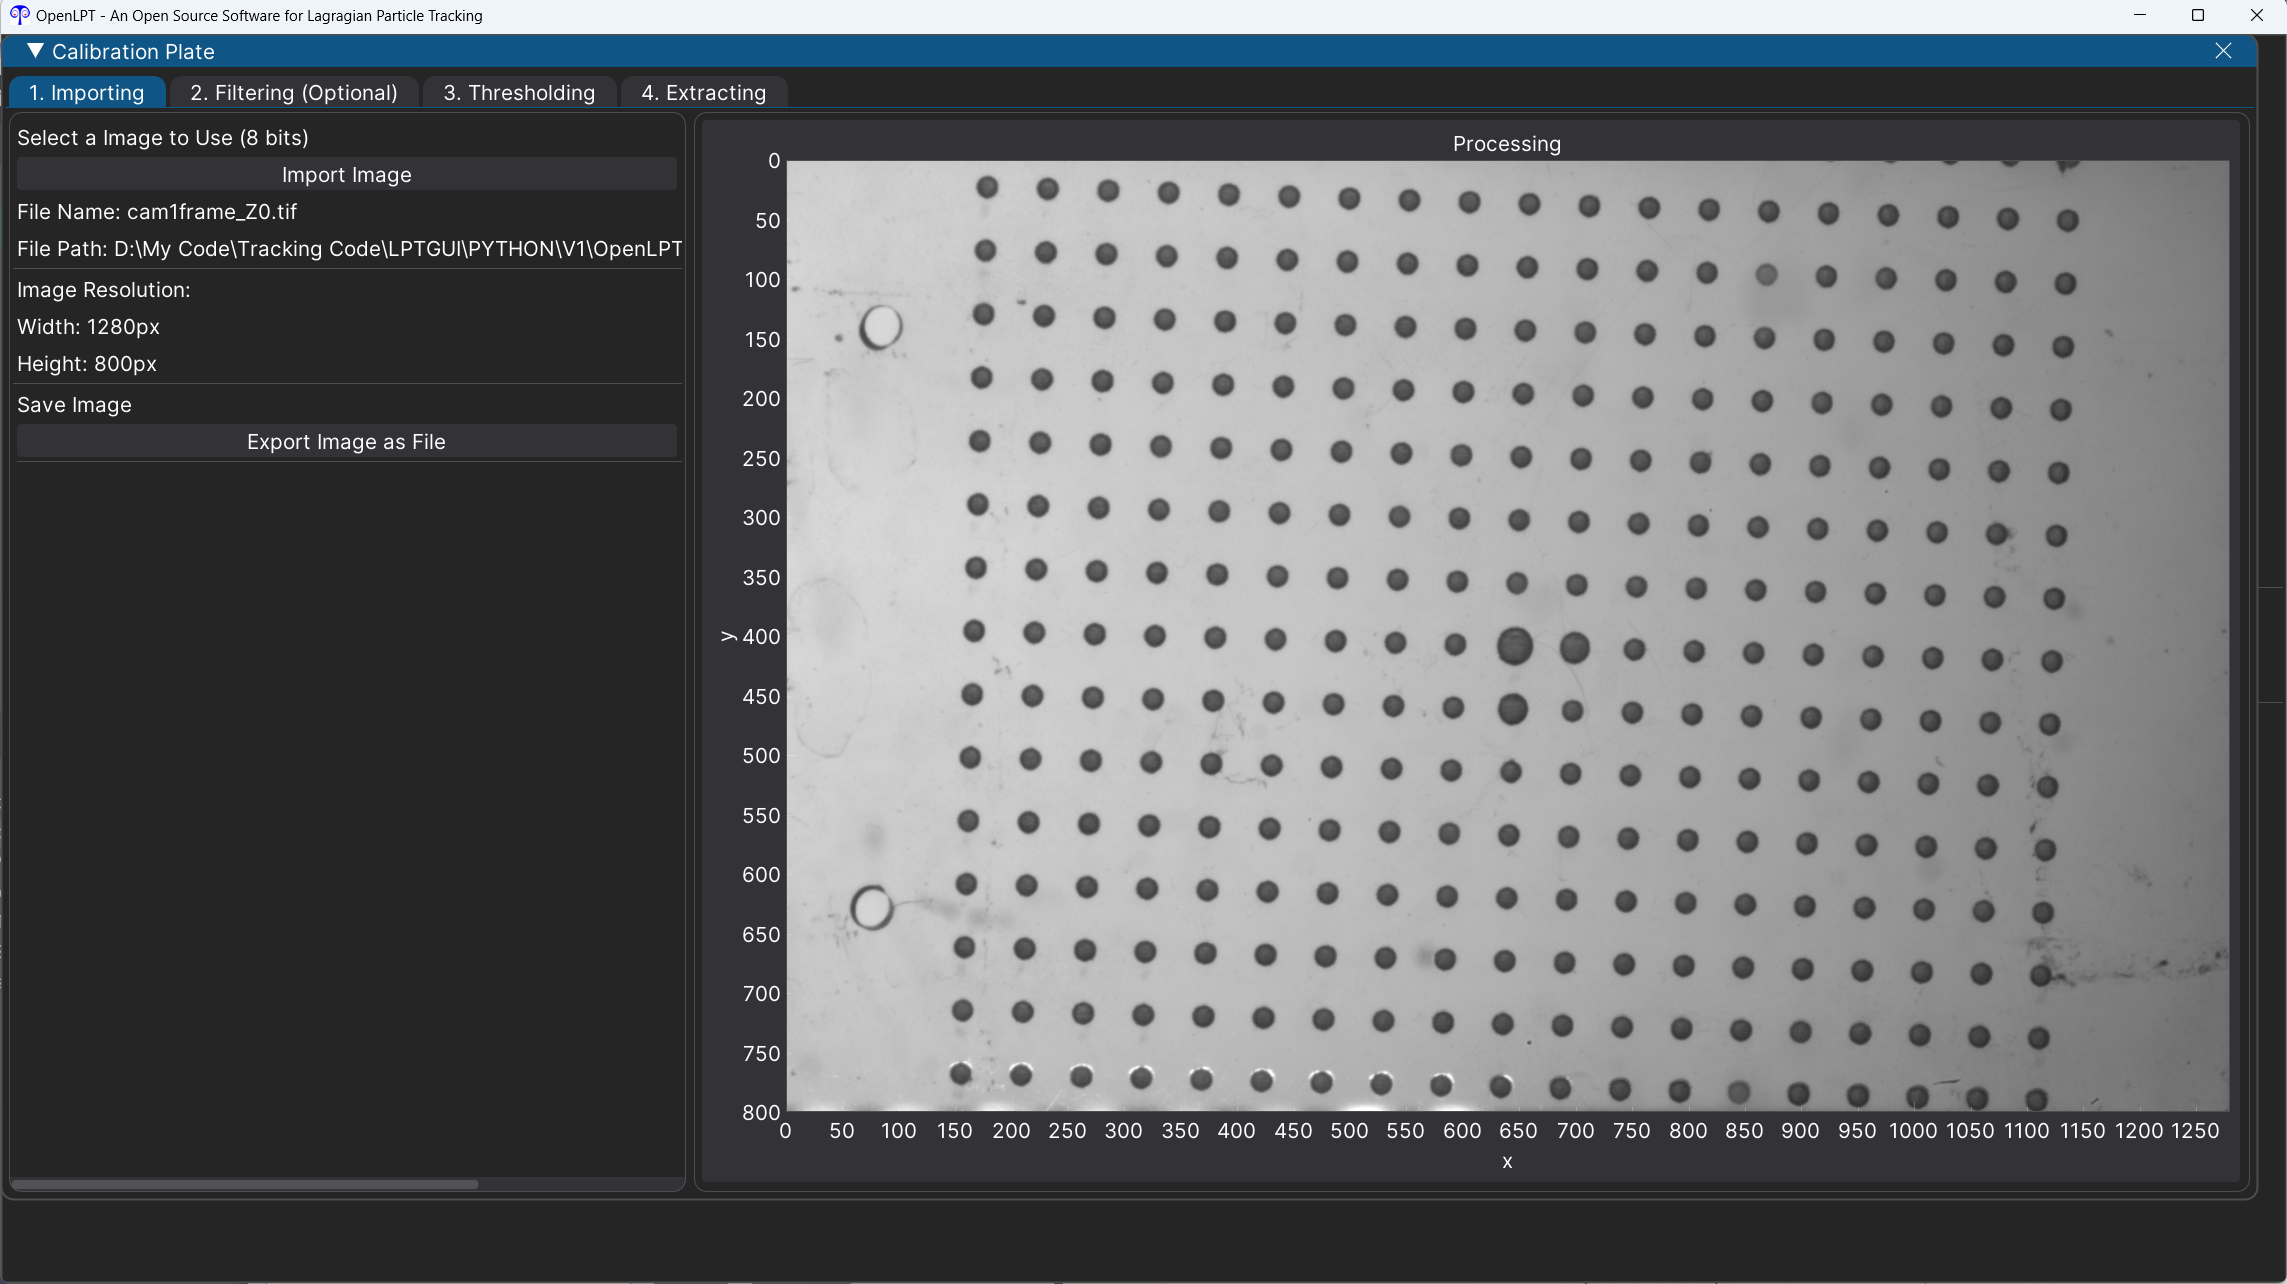
\includegraphics[width=\linewidth]{Fig/GUI_calibplate_import.png}
        \caption{The interface of the calibration plate method.}
        \label{fig:enter-label}
    \end{figure}
    
     \item \textit{Filtering (Optional)}\\
     \textcolor{blue}{Overview. }The functions on this page allows adjustments to the image for better processing.
     
     \begin{enumerate}
         \item Mask Area\\
         Users can press and drag the scroll wheel of a mouse to create a black or white rectangular area overlay. By checking the box next to "Mask Area," the overlays will appear on the image.

         \item Histogram Equalization\\
         This option redistributes the intensity values of the image's pixels to span the entire range of the intensity levels.

         \item Brightness\\
         This option allows adjustments of the image's average intensity pixels.
         
         \item Contrast\\
         This option allows adjustments of the intensity of distinctions between dark and light areas.

         \item Average Blur\\
         This option reduces image detail and noise by blending each pixel's value with the values of its neighboring pixels.

         \item Gaussian Blur\\
         This option works similar to average blur except by using a Gaussian function.

         \item Median Blur\\
         This option reduces noises while preserving edges of an image.\\
    \end{enumerate}
    
    \item \textit{Thresholding}\\
    \textcolor{blue}{Overview.} The functions on this page convert colored images into binary images. When the calibration dots are white, it can be identified better.
    \begin{enumerate}
        \item Global Thresholding\\
        This option allows the user to set an intensity value threshold (0-255), and intensity values that are larger or lower than this threshold are set to 1 and 0, respectively. 

        \item Invert Thresholding\\
        This option works similar to Global Thresholding, except the binarized image is inverted in that  intensity values that are larger or lower than this threshold are set to 0 and 1, respectively.

        \item Additional Thresholding Methods
        \begin{enumerate}
            \item Adaptive Mean Thresholding: Similar to Global Thresholding, but instead of using a single global threshold value for the entire image, this method calculates the threshold for smaller regions of the image. 

            \item Adaptive Gaussian Thresholding: Similar to Adaptive Mean Thresholding; uses a weighted sum of neighboring pixel values instead of a simple mean.

            \item Otsu's Binarization: A method that automatically computes the optimal threshold and separates the pixels into two clusters (works better after Gaussain Blur).\\
            
        \end{enumerate}
        
    \end{enumerate}
    \item \textit{Extracting}\\
    \textcolor{blue}{Overview}. This page works to extract the desired points on the uploaded image. 
    \begin{enumerate}
        \item Find Contour\\
        After entering the diameter range of the calibration dots on the image, the contours and centers can be extracted. The diameter can be estimated by checking the coordinate of mouse position shown on the bottom right corner. 

        \item Remove Wrong Points \\
        Users can remove wrong points by selecting the region on the image (dragging the left mouse button). To improve the number of identified points, user can go back to \textit{Filtering} page and mask out noisy area, or go back to \textit{Thresholding} page to adjust the threshold.
        
        \item Extract Plane Coordinates\\
        This step is to extract index position of each identified 2D points. 
        Users may choose a point on the image to serve as the origin, (0,0), and assign each axis index (top, bottom, left, and right) by counting the number of rows or columns. The positive or negative sign represents the direction of the real world coordinate. 

        \item Select four corners\\
        Four corners are used for identifying the surrounding axes, so they have to be on the same row or column. User can select the four corners of the calibration dots using left mouse button. The order of selection is Bottom Left$\rightarrow$Top Left$\rightarrow$Top Right$\rightarrow$Bottom Right.
        Additionally, users can define a threshold, which specifies the distance for whether to involve a point on the axis. If the distance between a point and the axis is less than the defined threshold, the point will be assumed to be located on the axis. 
        An example interface is shown in Fig.\ref{fig:GUI_calibplate_extract}.
        \begin{figure}[h]
            \centering
            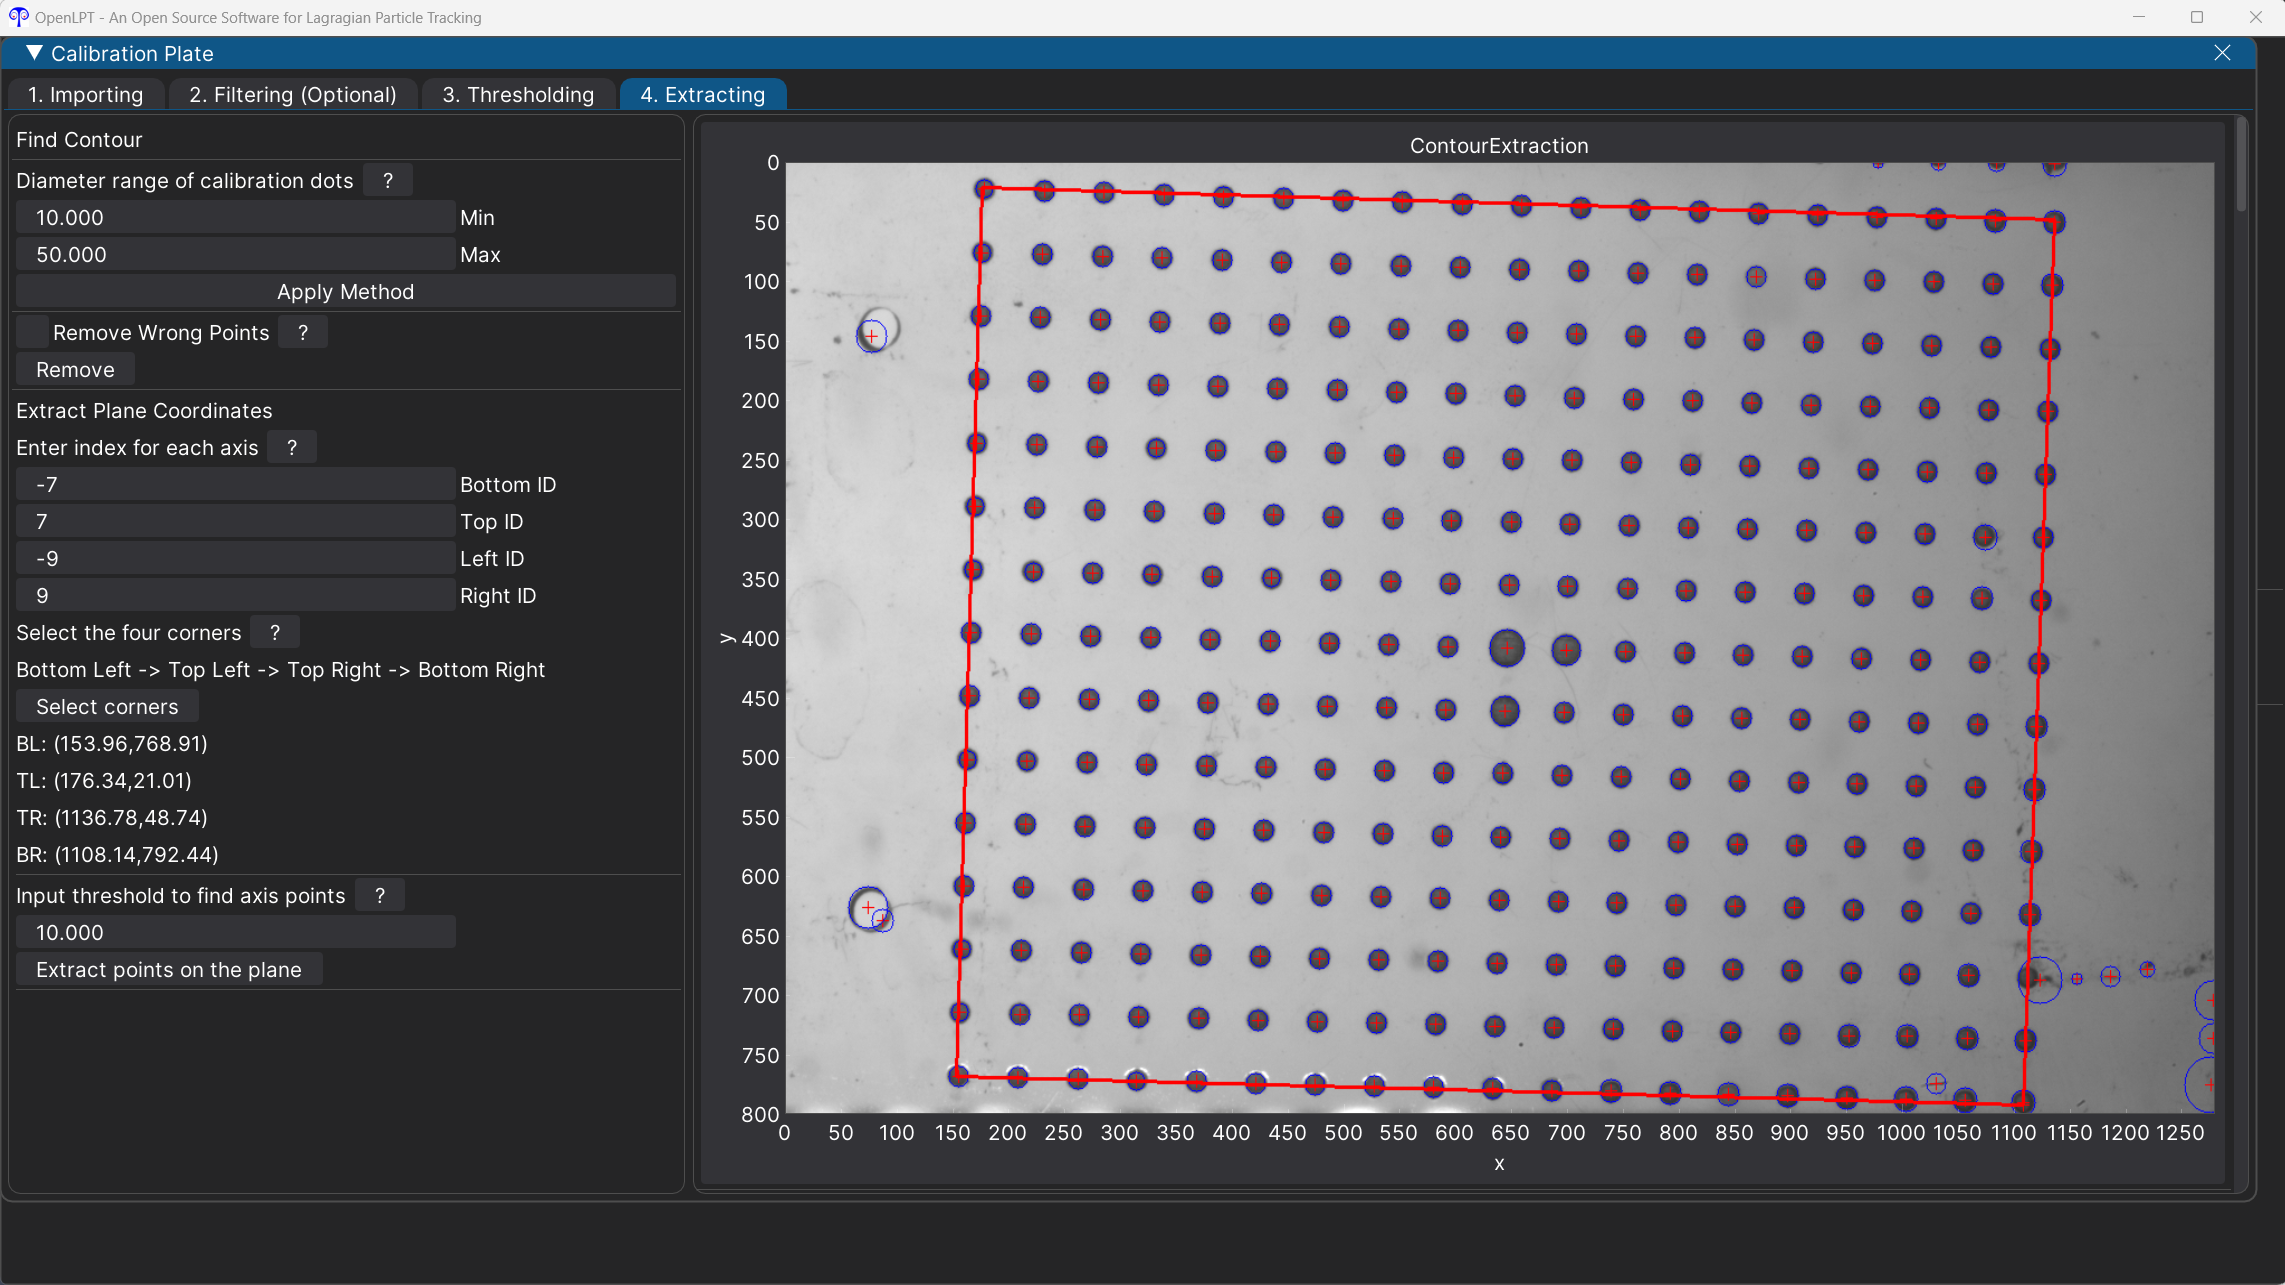
\includegraphics[width=\linewidth]{Fig/GUI_calibplate_extract.png}
            \caption{An image of the calibration plate with four corners selected to enclose the extracted points.}
            \label{fig:GUI_calibplate_extract}
        \end{figure}

        \item Extract World Coordinates\\
        Users are prompted to enter the depth of the calibration plate and the real-world distance between the calibration dots. Users should also indicate how the image's plane coordinates corresponds to the real-world coordinate system.

        \item Saving the document\\
        Save the work by clicking "Extract world coordinate". A sample output file is located at \file{images/opencvCalib.csv}.
        
        \end{enumerate}
         
    \end{enumerate}

\end{enumerate}

\subsection{Camera Model Selection}

In this step, the goal is to calibrate the camera parameters. If users already have the 2D positions and the corresponding 3D positions, step 1 can be skipped. Two camera models are supported including the \textit{pinhole} model and the \textit{polynomial} model. For 3D tracking, using the combination of both pinhole and polynomial camera models for different cameras is also supported. 

\begin{enumerate}
    \item Pinhole\\ 
    \textcolor{blue}{Overview. }The pinhole camera model is a model where a scene is obtained by projecting its 3D point coordinates into the image plane with appropriate transformations. It includes two steps: calibrate the camera intrinsic parameters (focal length and distortion factors), and calibrate the camera pose parameters (rotation matrix and translation vector).
    Note that for calibrating camera intrinsic parameters, users can put calibration plates at different angles to the camera and set them as the same 3D positions (use different coordinates). In that way, users can have a better estimation of those parameters. Additional information can be referred to OpenCV camera calibration steps. But users can use the same points that will be used for calibrating pose parameters.

    \begin{enumerate}
        \item Calibrate Camera Parameters\\
        Start by importing the image coordinates file generated from the calibration plate method. If the points are stored in multiple files, please select all of them. Then specify the image's width and height in pixels. There are several additional configurations to consider, including the following:
        \begin{enumerate}
            \item Fix Aspect Ratio: uses the same focal length in the x and y direction. \textbf{Usually set as True.}

            \item Fix Principal Point: sets the center point on the image the same as that of the camera. \textbf{Usually set as True.}

            \item Select a Distortion Model: three are three available models to choose from:
            \begin{enumerate}
                \item Zero: No distortion correction is applied. \textbf{Usually selected.}

                \item Radial: 2nd: Corrects common radial distortions using a simple model.

                \item Full: Applies comprehensive corrections for all types of distortions.
            \end{enumerate}
            
            \item Select the Axis Pointing Towards the Camera
        \end{enumerate}

        Finally, click "Run Calibration". An example result is shown in Fig.\ref{fig:GUI_pinhole_camcalib}.
            \begin{figure}[h]
                \centering
                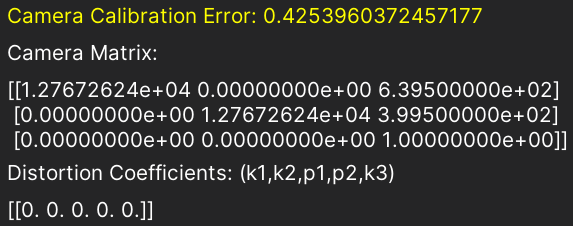
\includegraphics[width=0.8\linewidth]{Fig/GUI_pinhole_camcalib.png}
                \caption{An example result of camera calibration. The camera calibration error (in unit of pixels), camera matrix, and distortion coefficients are shown.}
                \label{fig:GUI_pinhole_camcalib}
            \end{figure}
        
        \item Calibrate Pose Parameters\\
        Start by importing the image coordinates file generated from the calibration plate method and then click "Run Calibration". The plot of projected 2D points based on the calibrated parameters is shown in Fig.\ref{fig:GUI_pinhole_posepts}. An example result of calibration is shown in Fig.\ref{fig:GUI_pinhole_posecalib}.
            \begin{figure}[h]
                \centering
                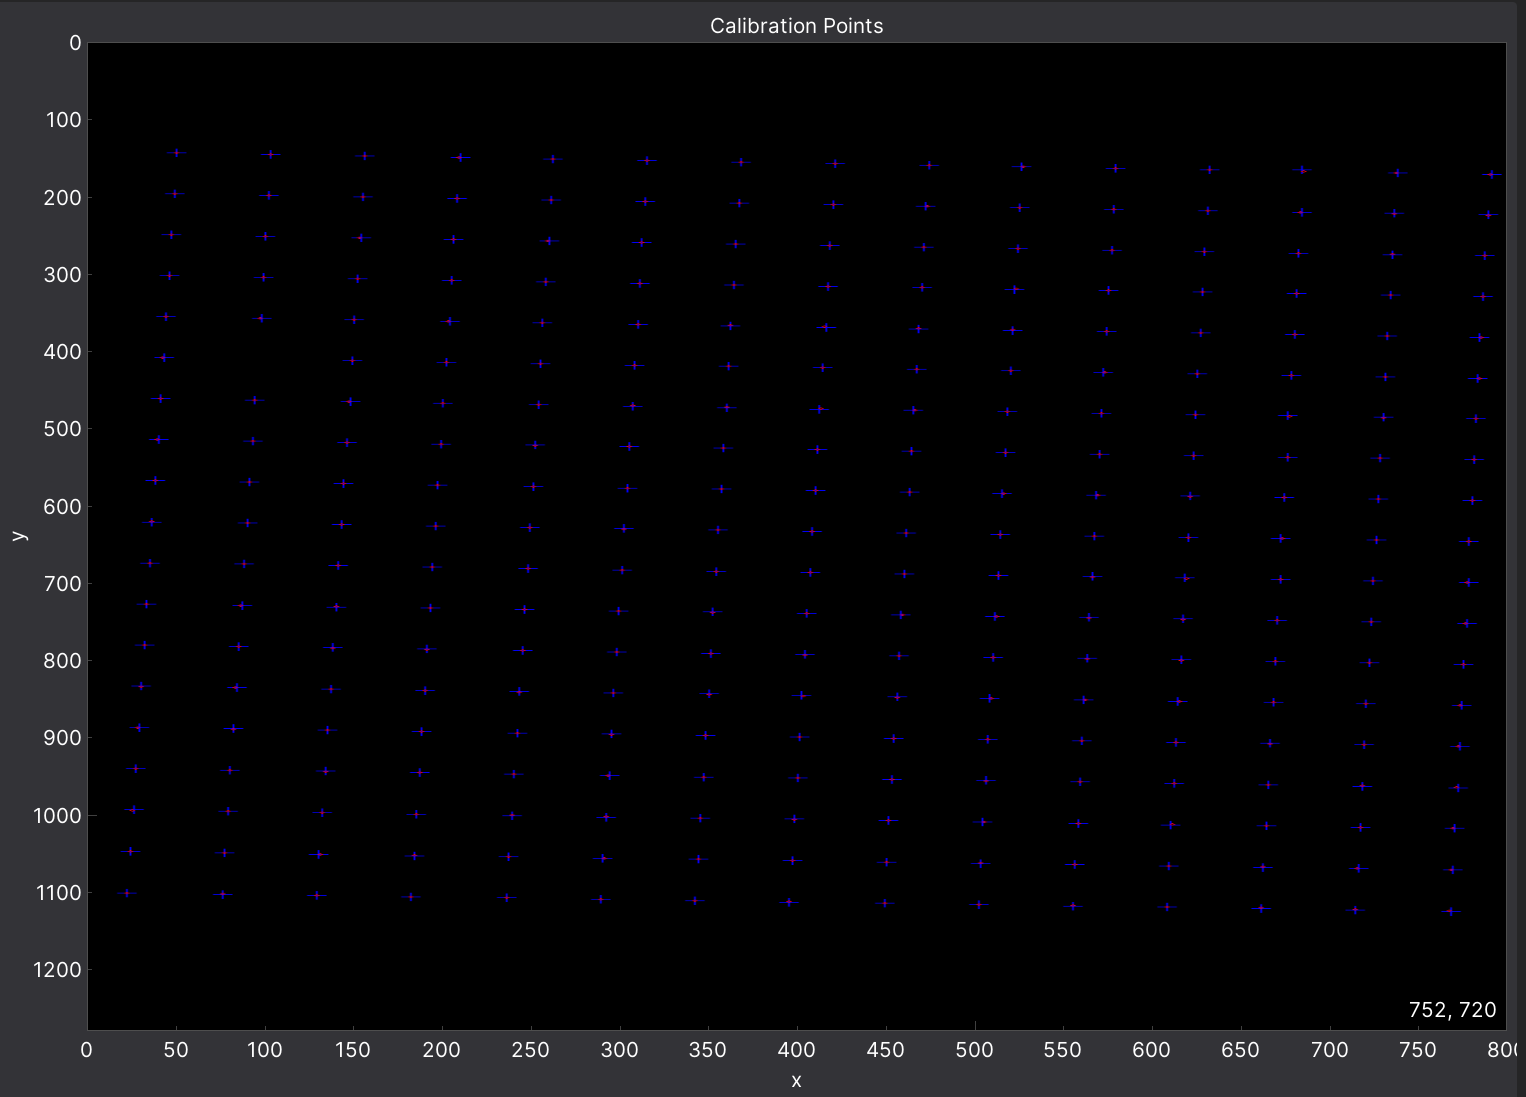
\includegraphics[width=\linewidth]{Fig/GUI_pinhole_posepts.png}
                \caption{A plot of calibration points generated from calibration of pose parameters.}
                \label{fig:GUI_pinhole_posepts}
            \end{figure}
            \begin{figure}[h]
                \centering
                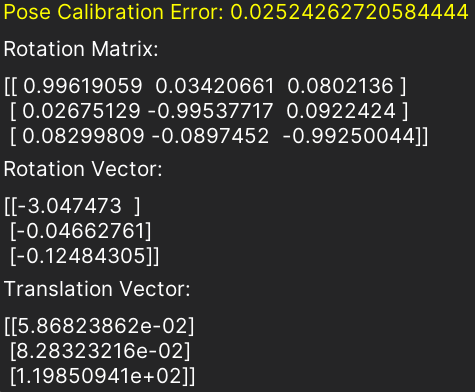
\includegraphics[width=0.8\linewidth]{Fig/GUI_pinhole_posecalib.png}
                \caption{The pose calibration error (in units of pixels), rotation matrix, rotation vector, and translation vector generated from the calibration.}
                \label{fig:GUI_pinhole_posecalib}
            \end{figure}

        \item Export Camera Parameters\\
        Users can save the work by clicking "Export". A sample camera file is located at \file{images/camFile/cam1.txt}.
        
    \end{enumerate}
    
    \item Polynomial\\
    \textcolor{blue}{Overview}. The polynomial camera model is optimal when the camera is at a large angle with respect to the transparent wall (acrylic) in front of the field of view, or that there are other sources of distortions. This method fits a polynomial that best relate 3D coordinates to 2D coordinates.
    
    \begin{enumerate}
        \item Polynomial Camera Calibration\\
        Start by importing the image coordinates file generated from the calibration plate method. Then specify the image's width and height in pixels. Then specify the order of polynomial (3-5 is recommended). An example of calibration result is shown in Fig.\ref{fig:GUI_poly_calib}.
        
        \begin{figure}[h]
            \centering
            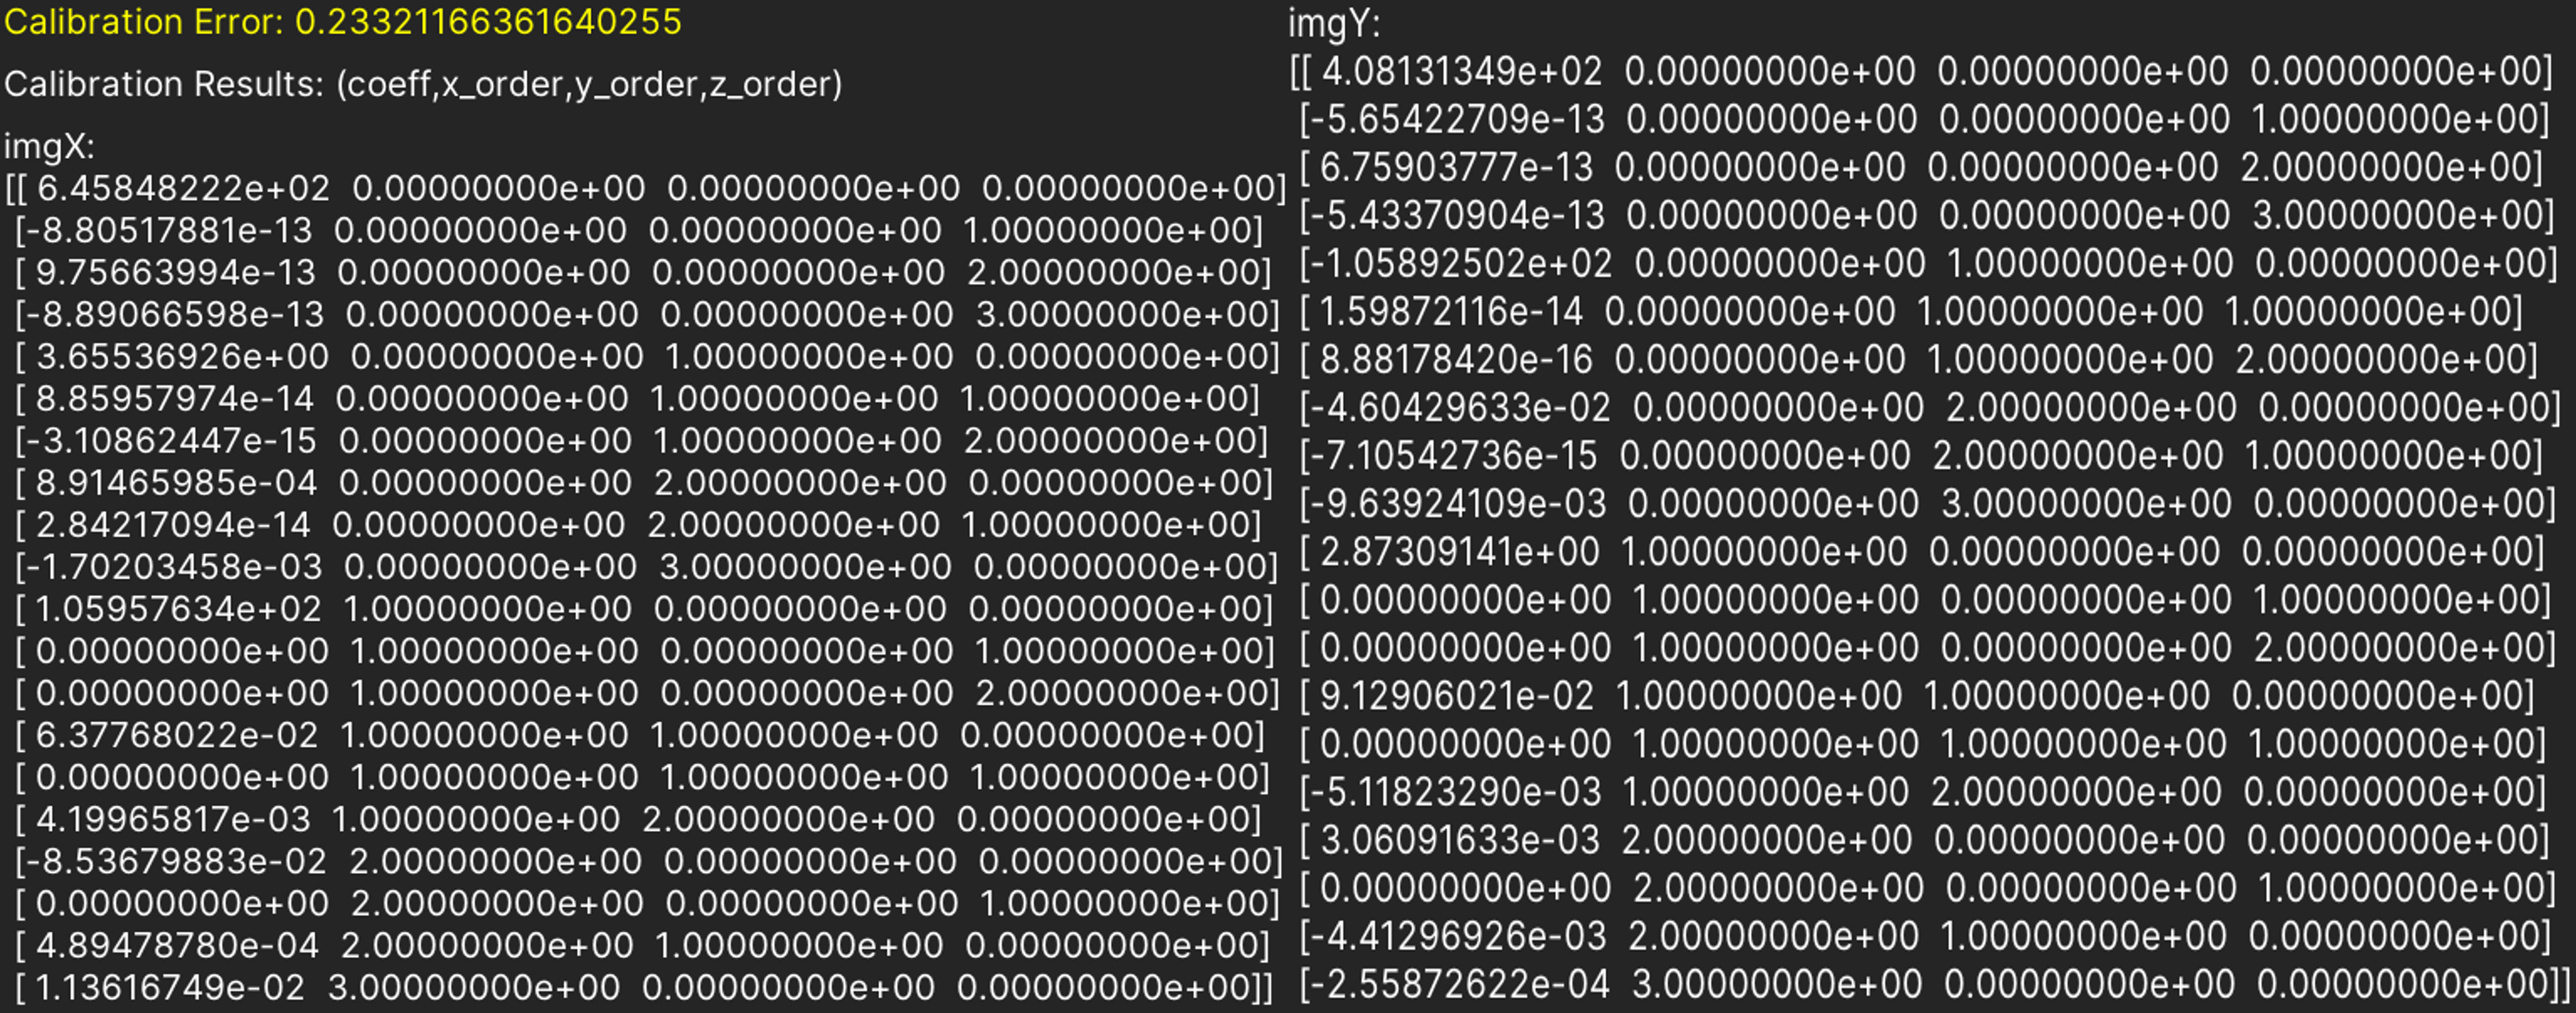
\includegraphics[width=\linewidth]{Fig/GUI_poly_calib.png}
            \caption{The generated results from polynomial calibration; the calibration error (in units of pixels) and the projected point coordinates are shown.}
            \label{fig:GUI_poly_calib}
        \end{figure}

        \item Select Reference Plane\\
        This step requires users to choose one of the three (x, y, and z) axis and specify two locations to create two reference planes. It is for creating a line of sight for a 2D point on the image. By calculating the corresponding 3D points on the two planes, a line of sight can be created. Therefore, this plane should be as parallel to the image plane as possible. For example, if the image x and y corresponds to the world coordinate x and y, then users should choose "REF\_Z" at the first step. The locations of these two planes are suggested to be set as the locations where the calibration plate have been placed.
        To save the work, click "Export Coefficients."
        
    \end{enumerate}
    
    
\end{enumerate}

\subsection{Image Preprocessing}
\begin{enumerate}
    \item Create Image Files (Optional)\\
    \textcolor{blue}{Overview}. In this step, the paths to all the images can be generated and saved to one file.
    \begin{enumerate}
        \item Select Image Main Folder\\
        Select the main folder containing all camera folders. The camera folders should have the same prefix ending with number and the order of number should be the same as the camera files (e.g. cam1, cam2, etc.). An example of extracted selected sub-folders is shown in Fig.\ref{fig:GUI_imgpre_subfolder}.
        \begin{figure}[h]
            \centering
            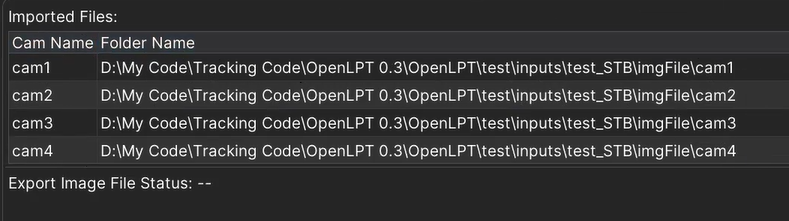
\includegraphics[width=\linewidth]{Fig/Screenshot (13).png}
            \caption{An example of selected image folders with their names listed on the left side and their respective paths listed on the right side.}
            \label{fig:GUI_imgpre_subfolder}
        \end{figure}

        \item Input Image Name Suffix\\
        Users should specify the image file suffix here (e.g. .tif). OpenLPT currently only supports reading .tif file but will support other formats in the future.

        \item Save Image File Path\\
        This option allows users to specify the image frames to be used for tracking. The first image frame in the folder would be the 0th image. If three frames are needed, then the range would be 0-2. To save the images, select a folder to store the files and click "Save".
        
    \end{enumerate} 

    \item Image Processing\\
    \textcolor{blue}{Overview}. This step is used for preprocessing the raw images. 
    
    \begin{enumerate}
        \item Import Image Path Files\\
        Import images by selecting the image path files created in the previous step.

        \item Image Processing
        \begin{enumerate}
            \item Preview Image\\
            To preview a specific image frame from the folders, specify the folder and the frame. An example of displayed image frame is shown below. 
            \begin{figure}[h]
                \centering
                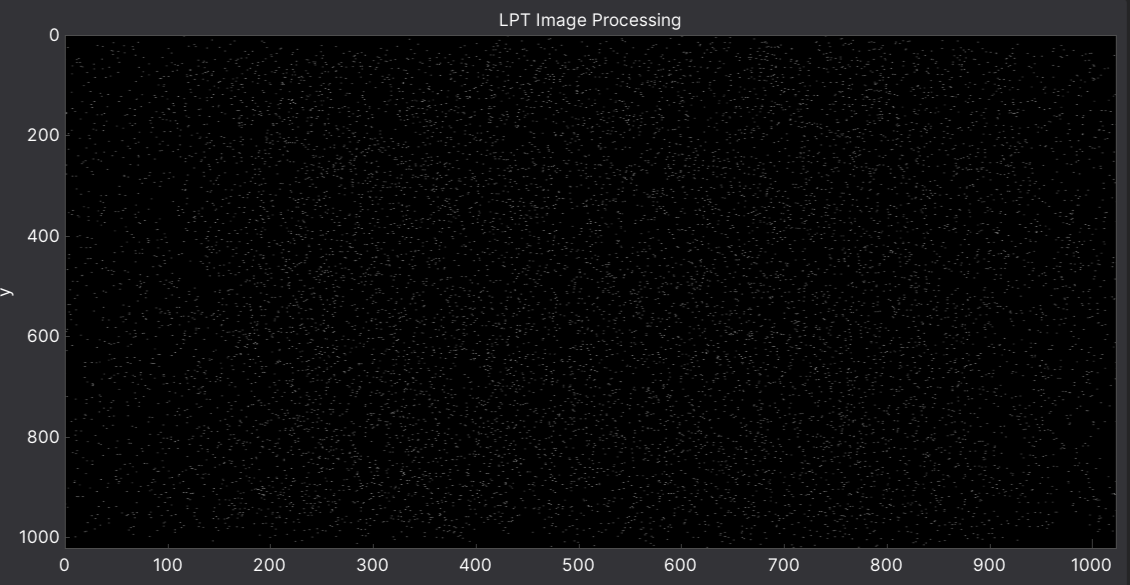
\includegraphics[width=\linewidth]{Fig/Screenshot (14).png}
                \caption{An image frame displaying the particles.}
                \label{fig:GUI_imgpre}
            \end{figure}

        \item Invert Image\\
        This function inverts the colors in the image. It is recommended to keep particles white and the background black. 

        \item Remove Background\\
        This function removes redundant objects in the background. Users should input the number of frames that they wish to have the backgrounds removed and the frame step (e.g. if the frame step input is 2, the code will analyze every other frame). 

        \item Brightness\\
        This function allows adjustments of the image's average intensity pixels.
         
        \item Contrast\\
        This function allows adjustments of the intensity of distinctions between dark and light areas.

        \item Intensity Range\\
        Adjusting the intensity range of the image can highlight the features in the image. 

        \item Sharpening Particles\\
        This function increases the brightness at the center of the particles in the image and enhance particle identification. 
        Gaussian Smooth Std and Mean Filter Size (odd) are parameters that adjust the image's quality. It is suggested to use the default values. 

        \end{enumerate}
        
    \item Run Batch
    \begin{enumerate}
        \item Select Output Folder\\
        Select a folder that will store the processed images. 

        \item Input Frame Range to Process\\
        Select the number of frames to store in the output folder (e.g. if you want to store the first twenty frames, input 0 and 19). 

        \item Parallel Threads\\
        Input the number of threads used for preprocessing the images in parallel.

        \item Hit "Run Batch" to export the selected files into the output folder. If successful, users should see "Finish!" at the bottom of the interface
    \end{enumerate}
        
    \end{enumerate}
\end{enumerate}



\subsection{OpenLPT analysis}
The goal of this step is to utilize OpenLPT for tracking objects. It includes sections for generating parameter files, running tracking algorithm and simple postprocessing interface. 

\begin{enumerate}
    \item Generate Configuration File (Optional)\\
    \textcolor{blue}{Overview.} This step is used for generating parameter files for OpenLPT. Users can also modify the sample configuration files provided in OpenLPT repository (\url{https://github.com/clockj/OpenLPT}), and skip this step.
        \begin{enumerate}
            \item Import camera files\\
            Import all the calibrated camera files from step 2.

            \item Import image path files\\ 
            Import all the image path files.

            \item Set main parameters\\
            Follow the instructions on the window and enter the parameters. Note that when setting the number of threads as zero, the code will utilize as many threads as possible for processing. A display of the window is shown in Fig.\ref{fig:GUI_lpt_mainParam}.

            \begin{figure}[h]
                \centering
                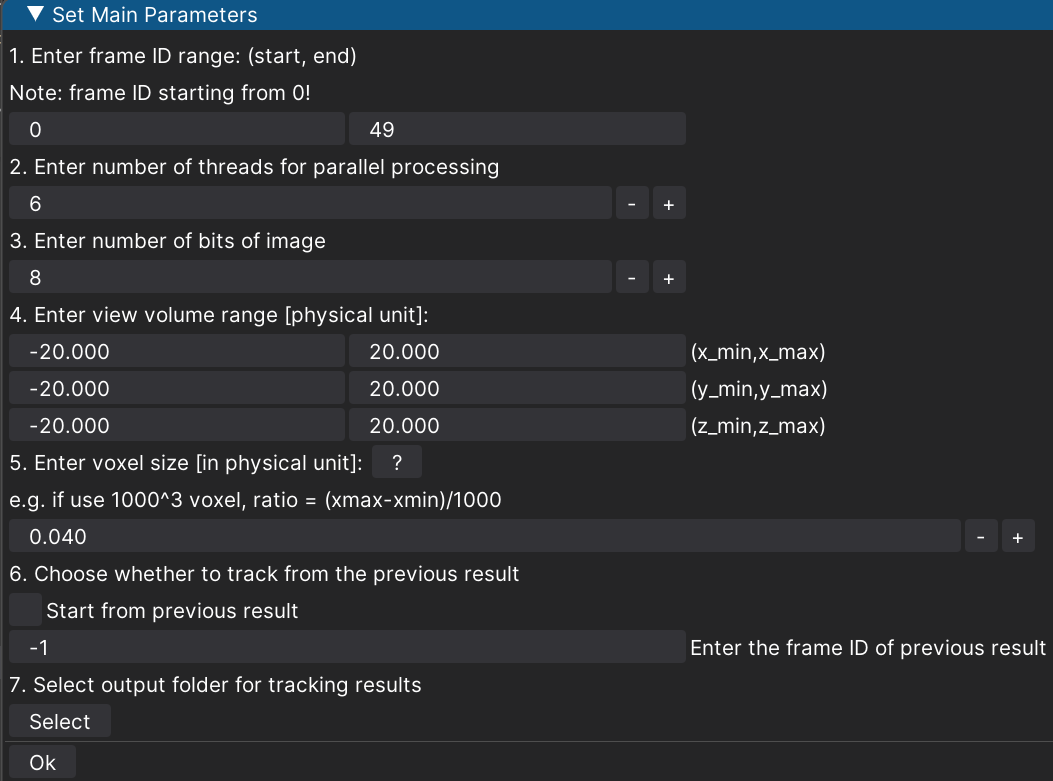
\includegraphics[width=\linewidth]{Fig/GUI_lpt_mainParam.png}
                \caption{A display of window for setting main parameters.}
                \label{fig:GUI_lpt_mainParam}
            \end{figure}

            \item Set object parameters\\
            This step is to set object parameters and add object types. Currently it only supports tracking of tracer particles, but implementation of spherical objects tracking will be implemented in the future. By adding more than one objects, it means the code will track all these objects at the same time. At each frame, it will first process the first object and then deal with the next by using the residue image. \\
            
            Follow the instructions on the window, and enter the parameters. A sample display of the window is shown in Fig.\ref{fig:GUI_lpt_tracerParam}. 
            Most of the parameters can be kept as the default, but users should check the following parameters. \\
            
            By setting the number of grids for the predictive field, users should make sure the grid size at each direction should be roughly the same. And the size of search radius should be comparable to the size of the grid. \\

            The number of IPR loops and number of shake loops can affect the processing speed. If the speed is too slow, users can consider adjusting these numbers. Besides, the speed is most sensitive to the 2D tolerance and users should make sure this value should be less than 2. If the number of tracks is too small, users and try increasing the 2D and 3D tolerances. By increasing the number of reduced cameras, more tracks can be found but the processing time will also go up.  \\

            By changing the intensity threshold, the number of identified particles will change. Users should modify this value based on the noise intensity and the image bits. In the next section, users can also check the performance 2D object identification. The 2D tracer radius is mainly used for shake-the-box algorithm. This algorithm will optimize the 3D position based on the window around the projected 2D position. The window size is two times of the radius.

            \begin{figure}[h]
                \centering
                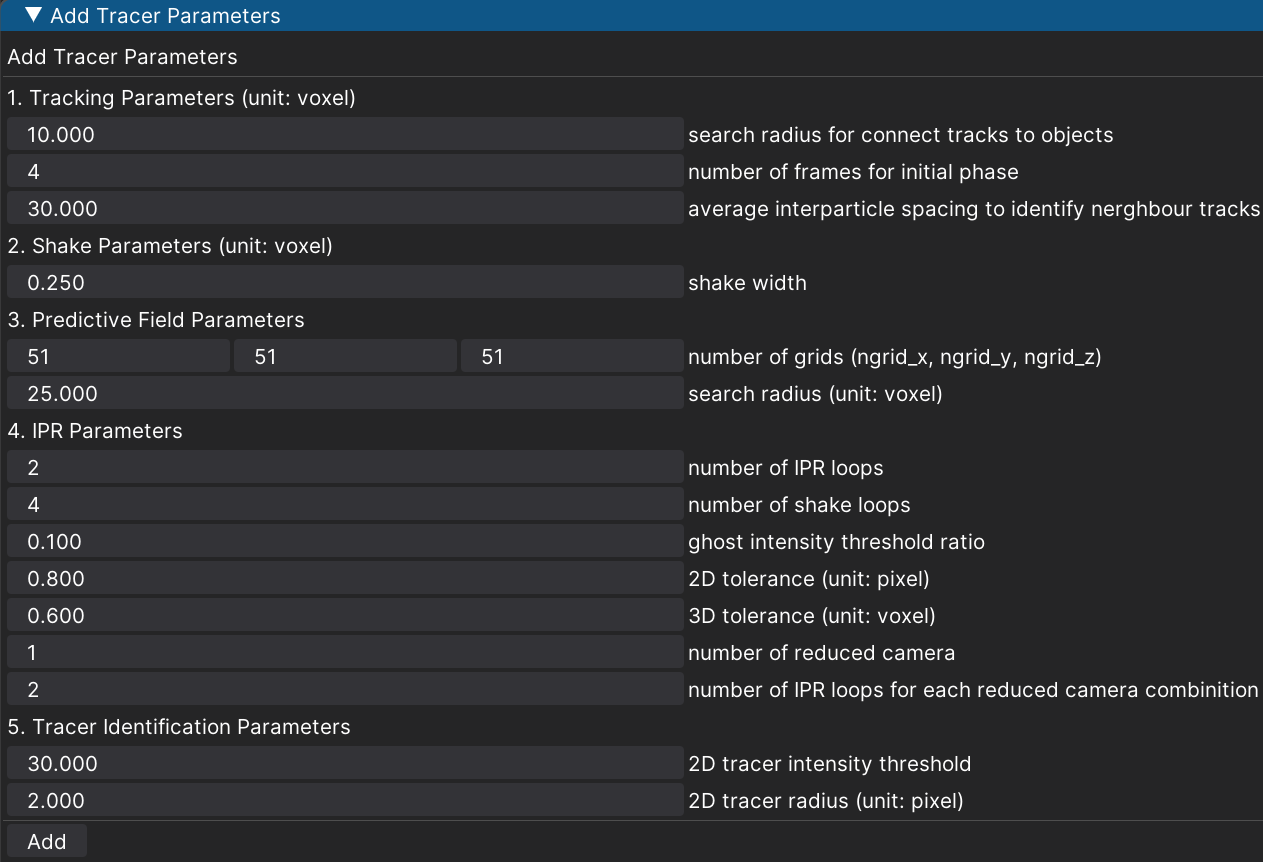
\includegraphics[width=\linewidth]{Fig/GUI_lpt_tracerParam.png}
                \caption{A display of window for setting tracer parameters.}
                \label{fig:GUI_lpt_tracerParam}
            \end{figure}

            \item Select export folder\\
            The configuration files will be saved to the chosen folder, and the generating status will be shown as "Finish!".
            
        \end{enumerate}

    \item Run OpenLPT    
    \begin{enumerate}
        \item Import main config file\\
        Import the generated main configuration file from the previous section. The default file name is "config.txt".

        \item Check Object Identification (Optional)\\ 
        Users can check the 2D object identification by using the generated parameters. In Fig.\ref{fig:GUI_lpt_run}, the red dots show the centers of identified particles. If the number of identified particles is too small or too larger, users can adjust the intensity threshold when setting the object parameters. Users can also try to improve the image quality during the preprocessing step.
        
        \begin{figure}[h]
            \centering
            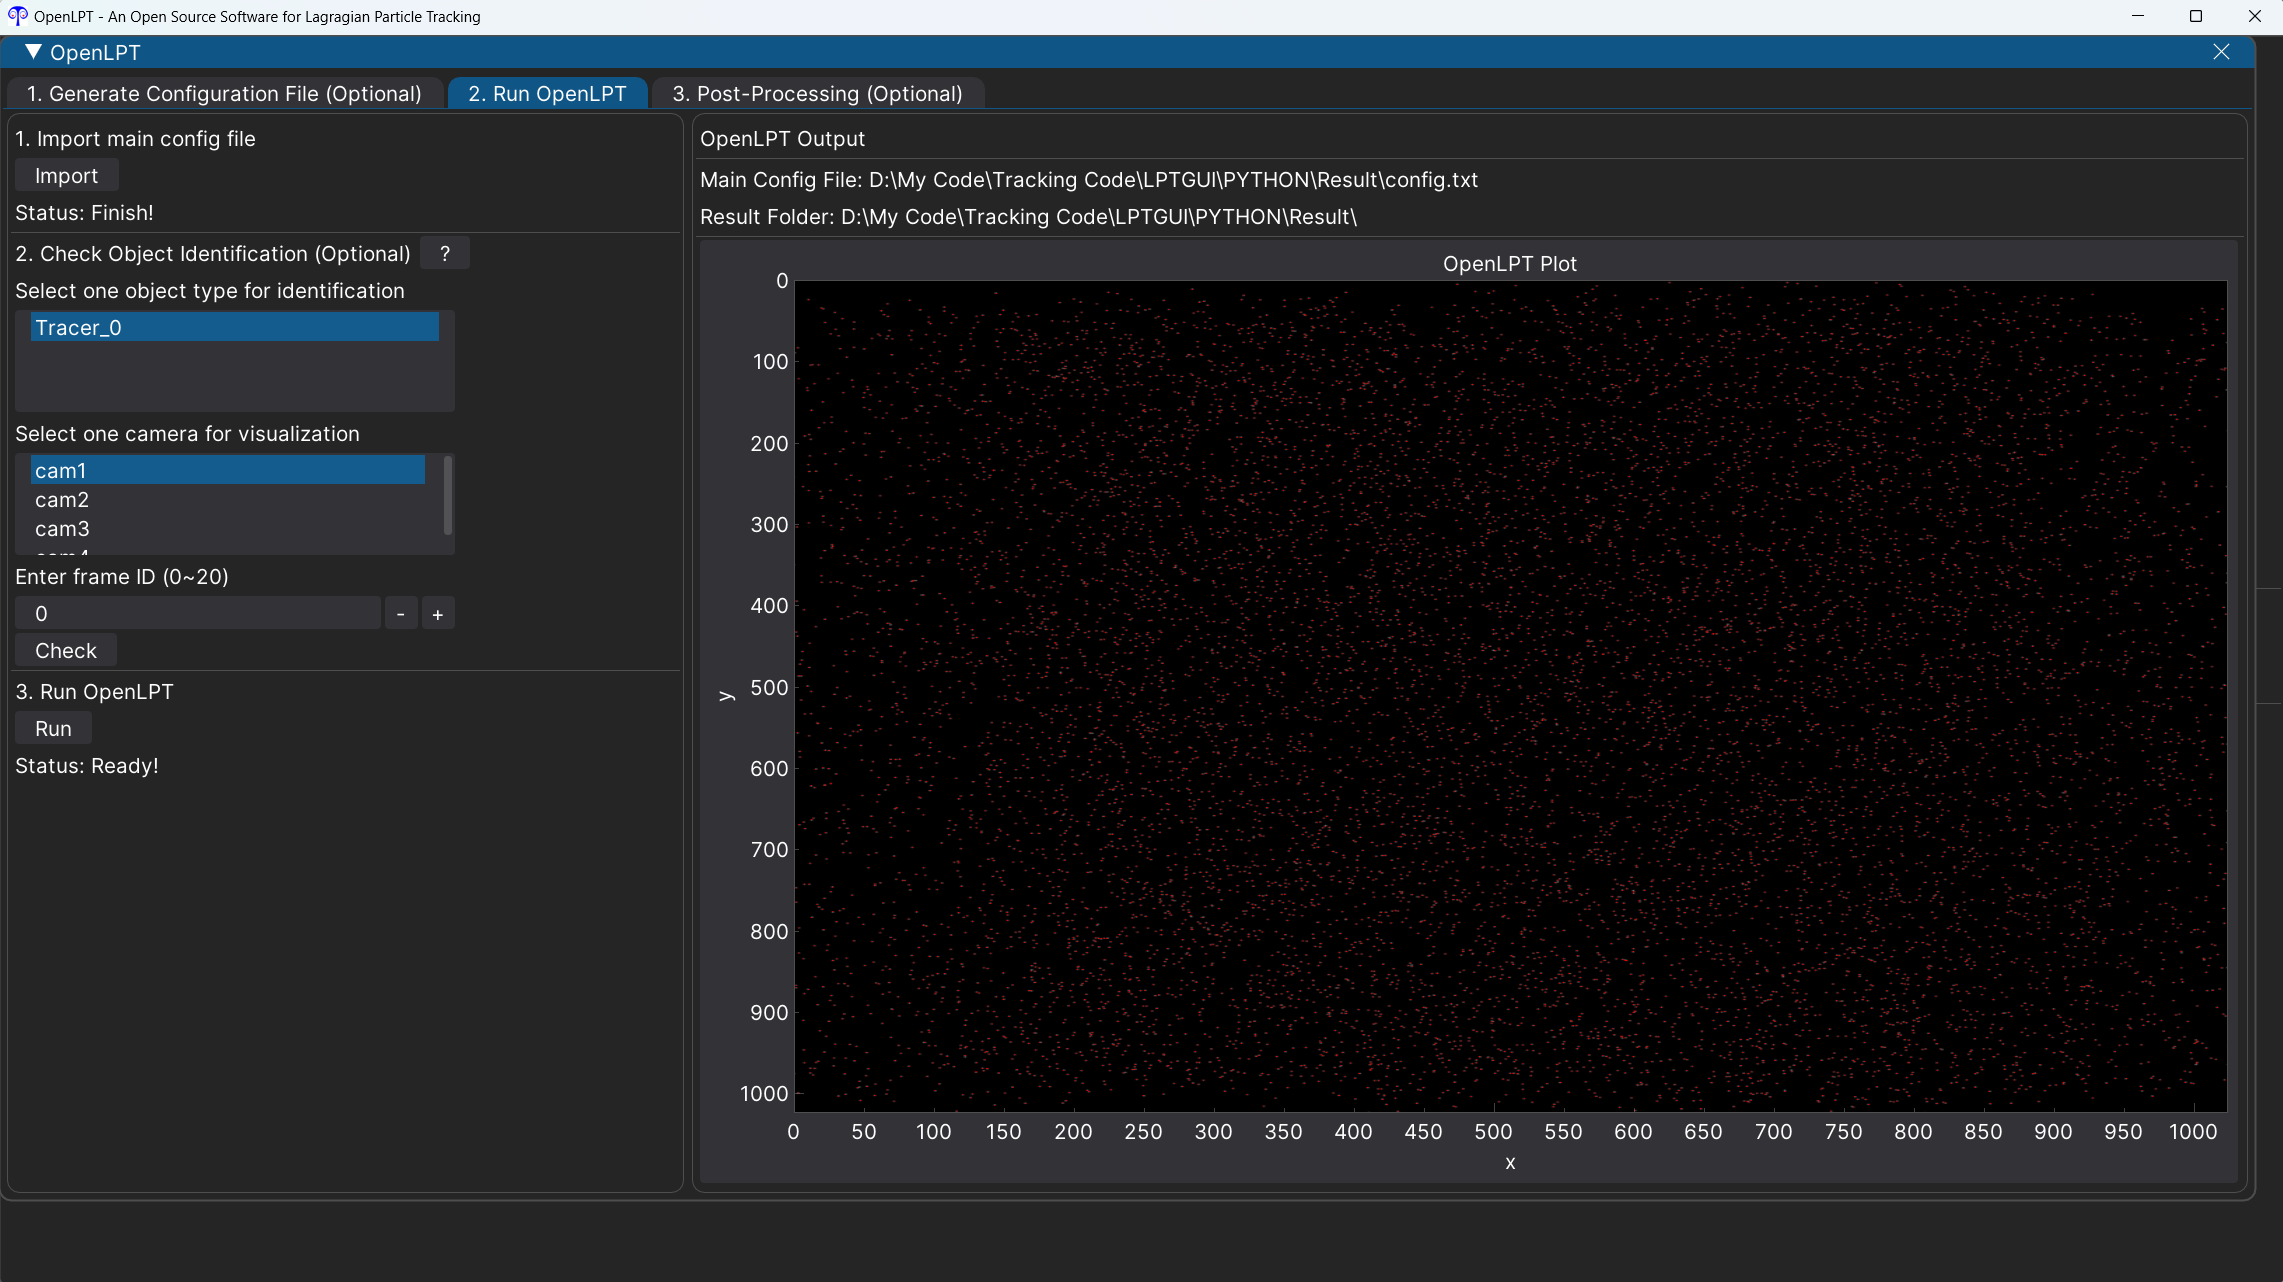
\includegraphics[width=\linewidth]{Fig/GUI_lpt_run.png}
            \caption{A sample of checking 2D object identification.}
            \label{fig:GUI_lpt_run}
        \end{figure}

        \item Run OpenLPT\\ 
        Users can click the "Run" button to start processing. The code outputs are shown in the command line. When it is finished, "Status" will be shown as "Finish!". All the output tracks will be stored in the folder \file{OutputTrack} of each object subfolder. 
    \end{enumerate}

    \item Post-Processing (Optional)
    Simple postprocessing features are implemented here, and more features will be added in the future. Fig.\ref{fig:GUI_lpt_post} shows a sample visualization of the postprocessing.

    \begin{figure}
        \centering
        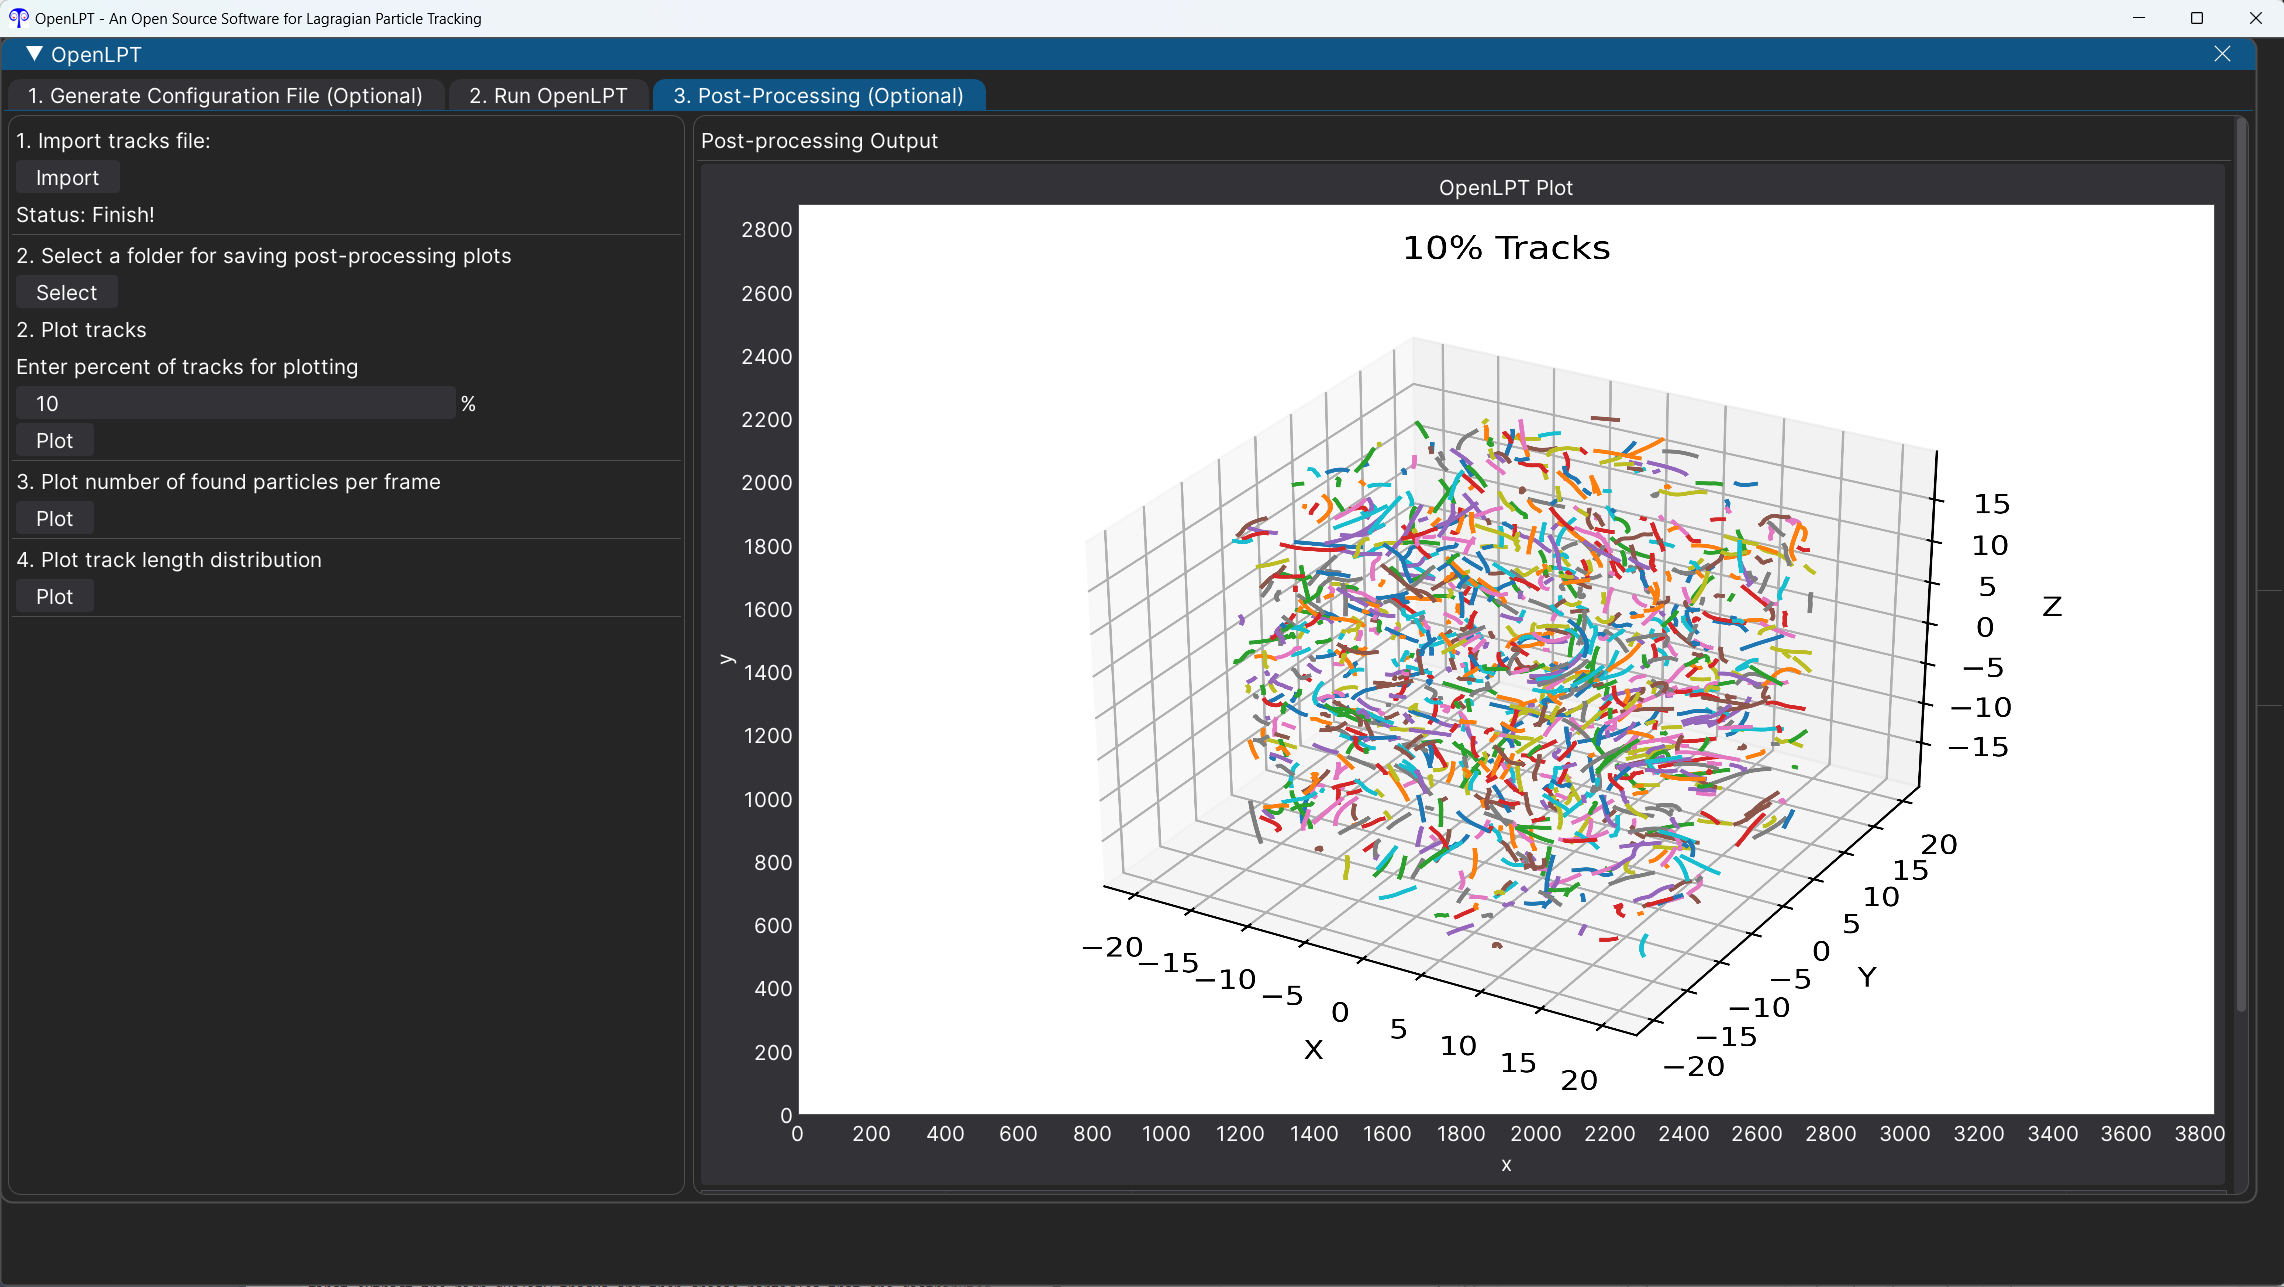
\includegraphics[width=\linewidth]{Fig/GUI_lpt_post.png}
        \caption{Sample visualization of processed tracks.}
        \label{fig:GUI_lpt_post}
    \end{figure}
    
\end{enumerate}



\subsection {Volume Self Calibration (VSC)}
In this step, users can optimize camera parameters based on the previous tracking results, which can increase the number of tracks and their accuracy. The code will first extract the high quality tracks and then choose particles that are distributed uniformly and use them for optimization.

\begin{enumerate}
    \item Import Camera Files\\
    Import all the calibrated camera files from step 2.

    \item Import Image Files\\
    Import all the image path files.

    \item Import Track Files \\
    Import the particle tracking files from step 4. By click the "Imported Tracks" button on the right panel, the tracks can be plotted onto the image as shown in Fig.\ref{fig:GUI_VSC_tracks}. A sample track file is located in \file{images/ActiveLongTrack50.csv}.

    \begin{figure}[h]
        \centering
        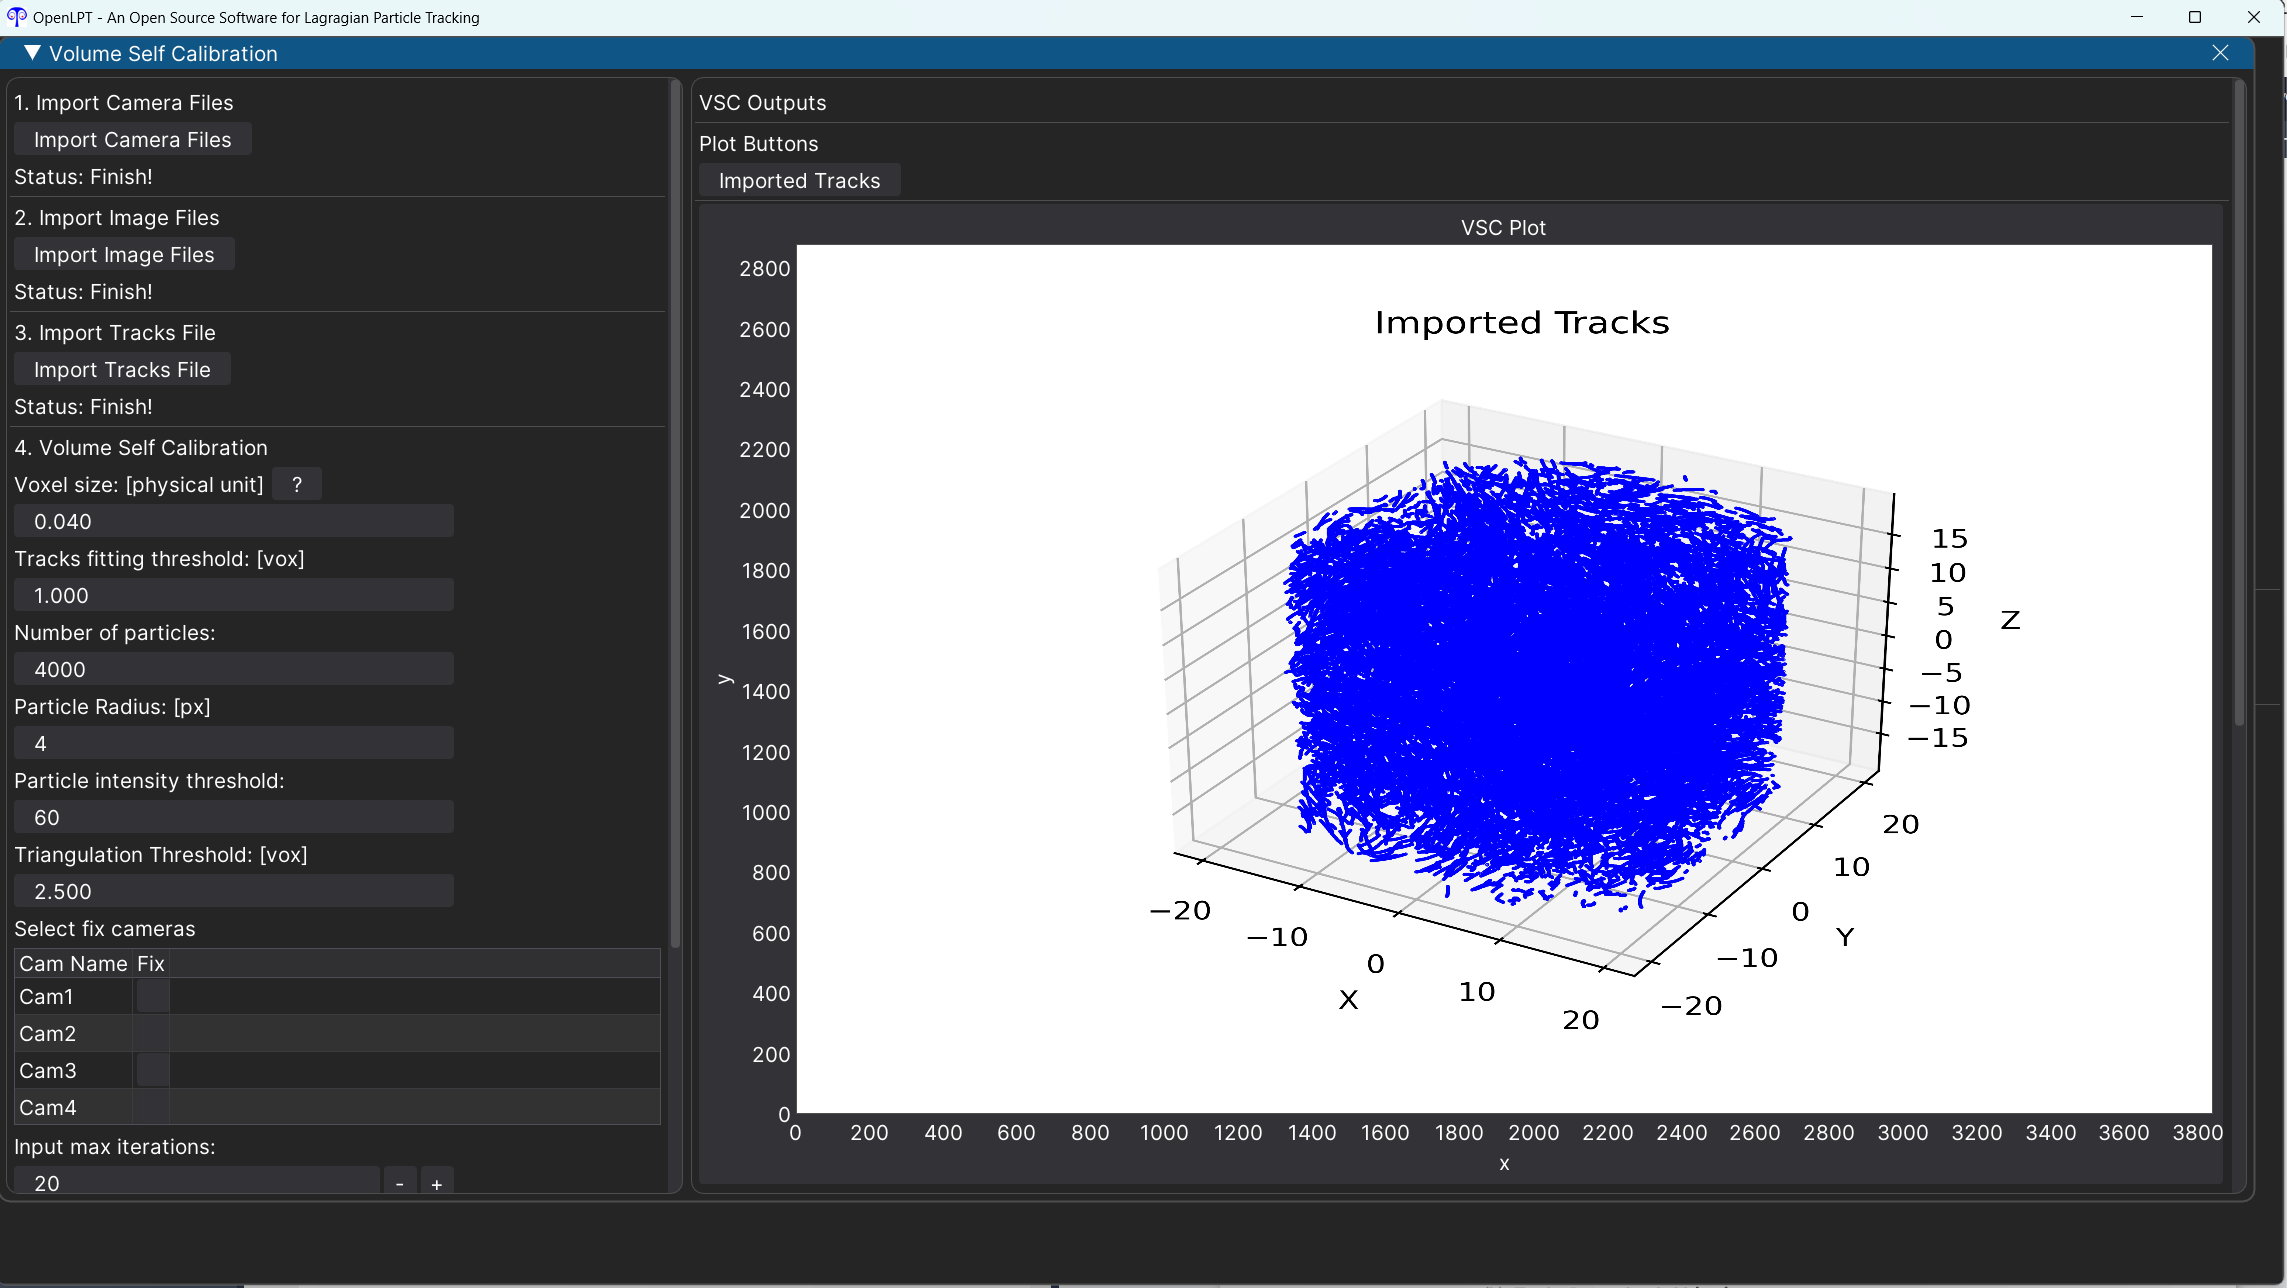
\includegraphics[width=\linewidth]{Fig/GUI_VSC_tracks.png}
        \caption{VSC imported tracks.}
        \label{fig:GUI_VSC_tracks}
    \end{figure}

    \item Volume Self Calibration\\
    \begin{enumerate}
        \item Voxel size\\
        Voxel size is the physical size of a voxel in the 3D space. This value is determined by the camera resolution and the view volume size. If the camera resolution is 1024x1024 and the view volume is [-20,20]x[-20,20]x[-20,20], this value could be set as 40/1000=0.04.
    
        \item Tracks fitting threshold [vox]\\
        The unit of this value is voxel, calculated as: view volume size/1000. This threshold is used to select smooth tracks by comparing the differences between the polynomial fitted positions and the original positions. 

        \item Number of particles\\
        Enter the number of particles to be used for optimization. It is usually set as 4000. During the VSC process, the number of particles that are uniformly distributed will be printed onto the command line output.

        \item Particle radius [px]\\
        It is used to search for 2D candidates on the image around the projected 2D locations from the 3D positions. It is usually set as 4 to increase the possibility to find the actual 2D candidates.

        \item Particle intensity threshold\\
        This threshold is used to identify the center of particles on images. If the center intensity is less this value, then it will not considered as a candidate.

        \item Triangulation threshold [vox]\\
        This threshold is used to filter out particles with high uncertainty (triangulation error). 
    
        \item Select fixed cameras\\
        It is used to fix the parameters of certain cameras if users do not want to optimize the parameters of the chosen cameras.

        \item Input max iterations\\
        Enter the maximum iteration steps for the optimizer.

        \item Input convergence tolerance\\ 
        The optimizer will stop when the change of parameters is smaller than this tolerance.

        \item Hit "Run Batch" to export the selected files into the output folder. If successful, users should see "Finish!" for all the stages.
    \end{enumerate}
    
    Users can plot the loss history during the optimization by clicking the "Loss" button on the right panel. Loss is measured by the mean triangulation error of all the chosen particles. The loss distribution can also be compared with the one before optimization by clicking "Error Histogram" as shown in Fig.\ref{fig:GUI_VSC_errhist}. The 3D positions before and after optimization can be visualized by clicking "Selected Particles". 

    \begin{figure}[h]
        \centering
        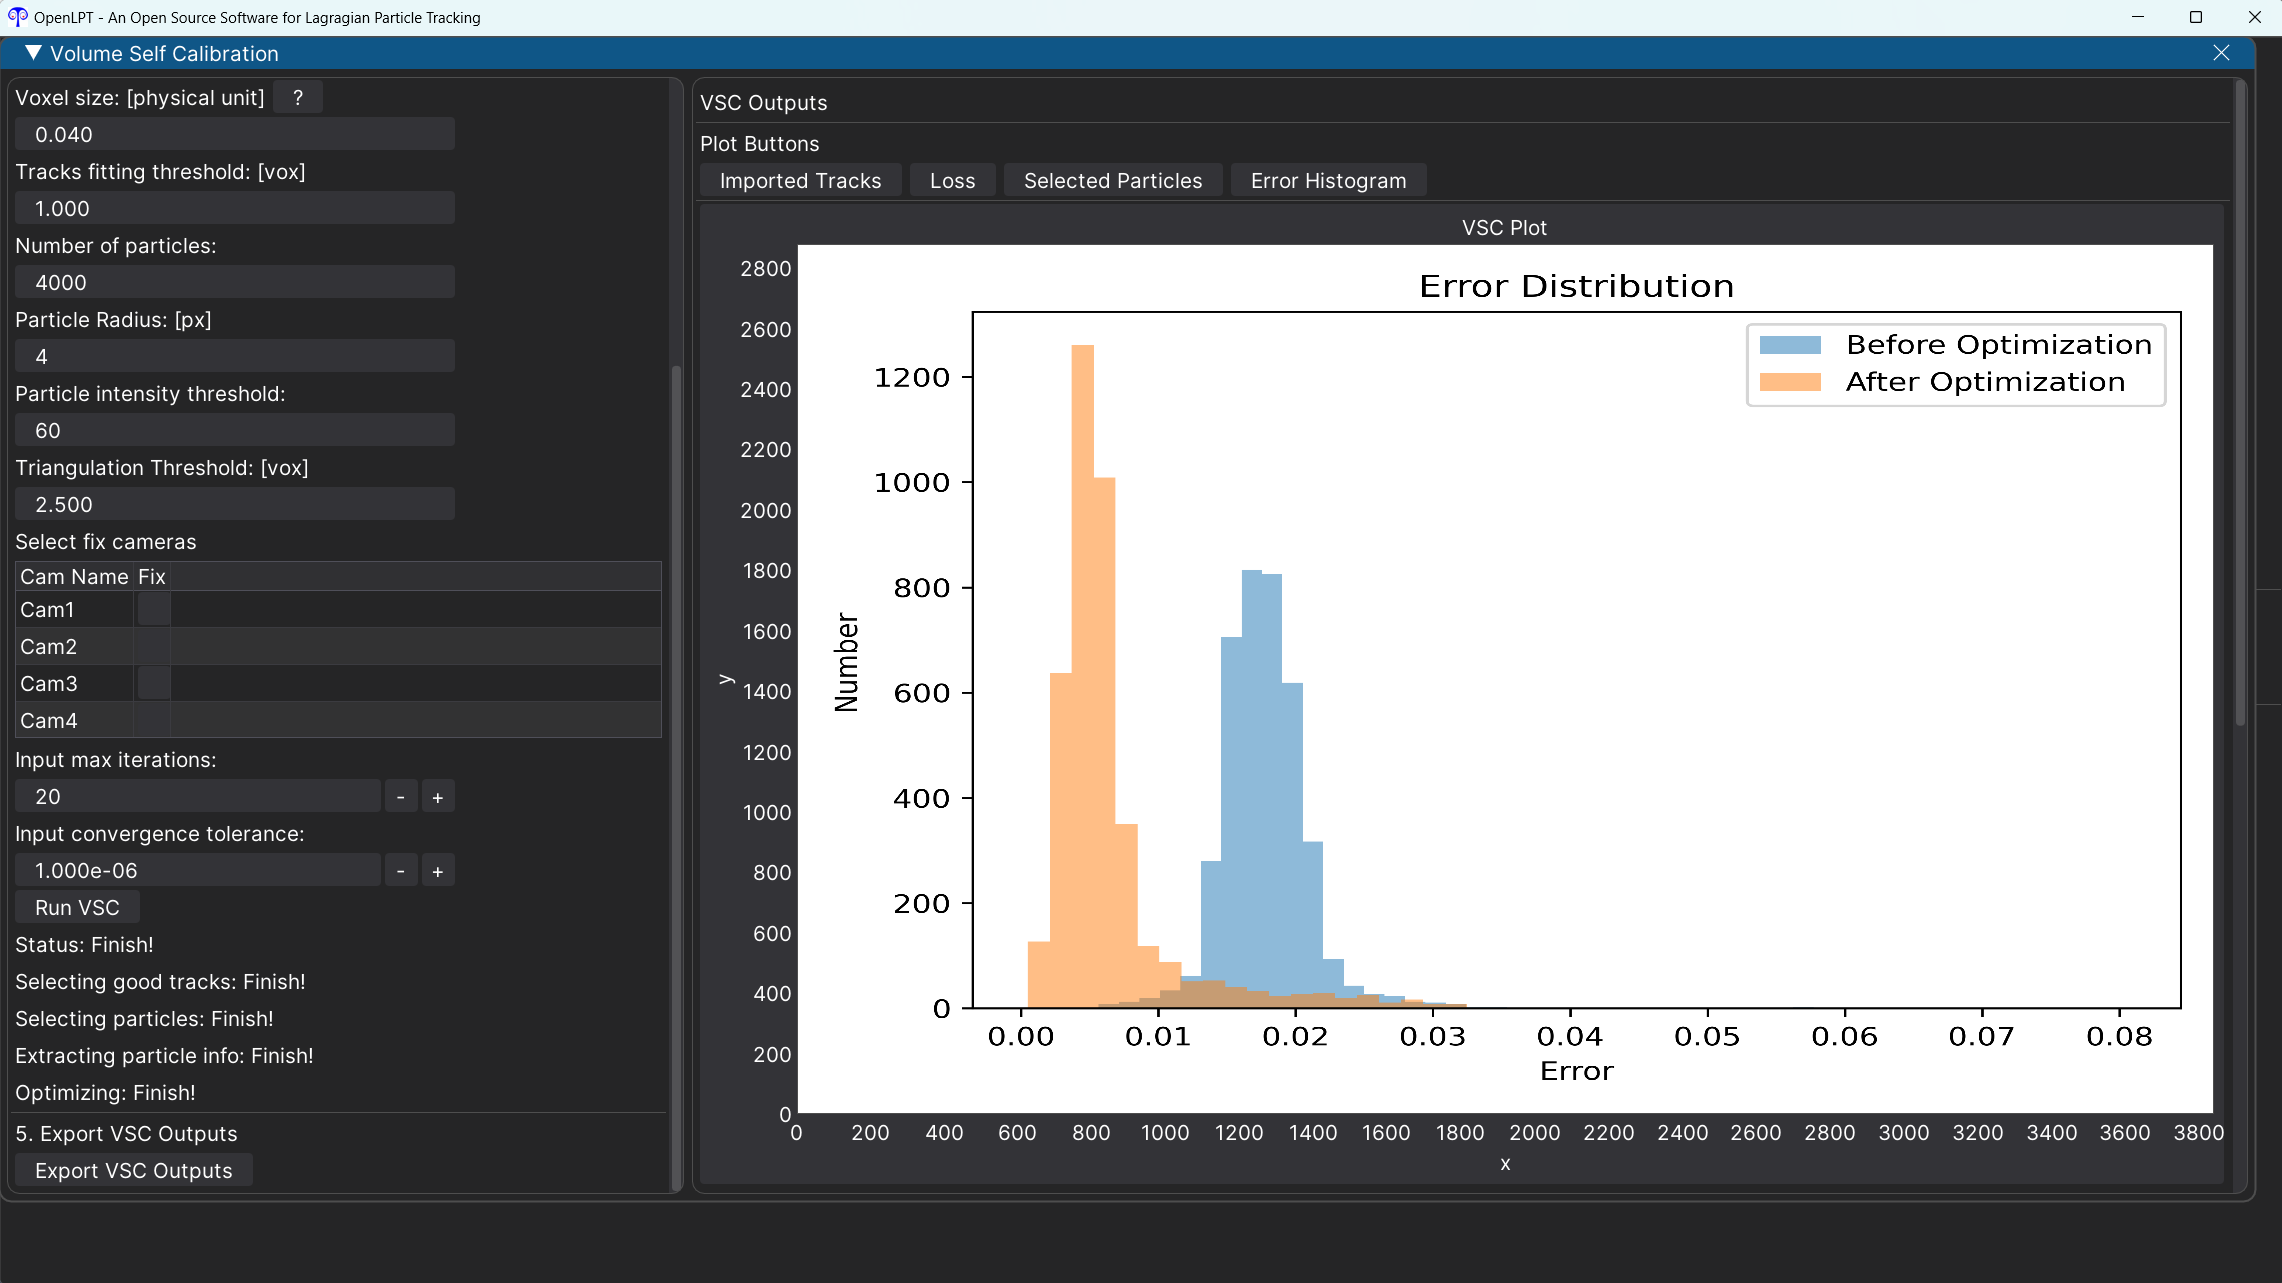
\includegraphics[width=\linewidth]{Fig/GUI_VSC_errhist.png}
        \caption{PDF of triangulation error before and after optimization.}
        \label{fig:GUI_VSC_errhist}
    \end{figure}
    
    
\end{enumerate}




\section{References}
\bibliographystyle{plain}
\bibliography{ref}

\end{document}
